\documentclass[11pt,a4paper]{article}
\usepackage[utf8]{inputenc}
\usepackage[T1]{fontenc}
\usepackage{lmodern}
\usepackage{geometry}
\usepackage{booktabs}
\usepackage{amsmath}
\usepackage{amssymb}
\usepackage{graphicx}
\usepackage{hyperref}
\geometry{margin=1in}
\setcounter{tocdepth}{3}

\title{Coursework Report: PPO and SAC+HER for RoboCasa Manipulation}
\author{\small BOUCNEAU Nathan, HORDOIR Stéphane, LATOUNDJI Mourad, ZHANG Chengbo}
\date{\today}

\begin{document}
\maketitle

\begin{abstract}
This report presents a unified study of two reinforcement learning pipelines for RoboCasa long-horizon manipulation: (i) PPO with dense reward shaping and (ii) SAC with Hindsight Experience Replay (HER) plus curriculum learning. We evaluate both methods on related apple pick-and-place tasks (\textit{apple-to-cabinet} and \textit{apple-to-bowl}) and focus on the gap between intermediate skill acquisition and final-task completion. The two lines do not fail in the same way. PPO with shaping reaches strong grasping but often stalls on \emph{carrying} the apple into a stable bowl configuration: metrics show grasp--place--success gaps consistent with transport and terminal-alignment limits even after reward rebalancing toward transport. SAC+HER under curriculum instead learns spatial approach and placement phases relatively well, then breaks down when the task explicitly requires \emph{release}: success collapses in the gripper-open phase while diagnostics show opening far from the goal. Both point to compositional manipulation difficulty, but the dominant training bottleneck is transport-centric for PPO and release-centric for SAC+HER in the reported runs.
\end{abstract}

\tableofcontents
\clearpage

\section{Introduction}
Sparse-reward robotic manipulation remains difficult because informative feedback is delayed and success conditions are compositional. In RoboCasa pick-and-place settings, an agent must jointly solve reach, grasp, transport, release, and post-release stabilization. When terminal reward is rare, training often collapses into partial behaviors.

To study this challenge, we compare two practical strategies used in this project:
\begin{itemize}
    \item \textbf{PPO + reward shaping}: dense progress rewards and versioned reward engineering (v1--v3).
    \item \textbf{SAC+HER + curriculum}: hindsight relabeling and phased difficulty scheduling.
\end{itemize}
\noindent The report goal is to compare where each method works, where each fails, and how those failure modes differ as well as what structural task features underlie both.

\section{Task Setup and Evaluation Criteria}
\subsection{Manipulation Tasks}
We consider two related tasks:
\begin{itemize}
    \item \textbf{Apple-to-Cabinet (apple-to-cab):} pick an apple from a counter and place it into a cabinet region.
    \item \textbf{Apple-to-Bowl (apple-to-bowl):} pick an apple from a counter and place it into a bowl.
\end{itemize}

\subsection{Success Definition and Transfer Difficulty}
The two tasks share a pick-transport-place structure, but differ in terminal constraints. The bowl task requires both successful placement and gripper disengagement, so any algorithm must eventually solve release as well as carriage. In practice, logged metrics and videos in this report suggest that PPO-shaped training often lags on \emph{carry-to-success} while SAC+HER under curriculum lags most visibly on \emph{release timing} once placement phases are learned. Policies transferred from apple-to-cab may preserve grasp and transport skills yet still underperform on final success in apple-to-bowl.

\subsection{Metrics}
To diagnose stage-wise learning rather than only final success, we track:
\begin{itemize}
    \item \texttt{success\_rate}, \texttt{place\_success\_rate}, \texttt{grasp\_success\_rate},
    \item closest-approach and, for SAC+HER bowl runs, gripper open- and release-distance summaries (OpenD/ReleD-style aggregates),
    \item episode reward trends (\texttt{ep\_rew\_mean}) for within-run dynamics.
\end{itemize}

\section{Methods}
\subsection{Method A: PPO with Reward Shaping}
\subsubsection{Objective}
We use PPO with an MLP policy and clipped policy updates. PPO optimizes:
\[
\mathcal{L}^{\text{CLIP}}(\theta) =
\mathbb{E}_t\left[
\min\left(r_t(\theta)\hat{A}_t,\,
\text{clip}(r_t(\theta), 1-\epsilon, 1+\epsilon)\hat{A}_t\right)
\right].
\]

\subsubsection{Shaping Design}
The shaped reward augments sparse environment reward with dense terms for:
\begin{itemize}
    \item contact and grasp acquisition,
    \item lift and transport progress,
    \item release and placement events,
    \item final success bonus.
\end{itemize}
For state labeling, v2/v3 do not directly use RoboCasa's default \texttt{OU.check\_obj\_grasped}. Instead, they use a task-specific robust grasp check and then define a stricter effective \texttt{grasped} state through additional gating (e.g., stability/transportability conditions). This redefinition is used consistently by reward logic and episode metrics.
The implementation also logs atomic metrics such as \texttt{contact\_success\_rate}, \texttt{grasp\_success\_rate}, \texttt{grasp\_lift\_success\_rate}, and \texttt{place\_success\_rate} to inspect stage-wise learning.

\subsubsection{Versioned Progression (v1--v3)}
The shaping pipeline uses a lightweight reward-curriculum mechanism across v1--v3. Specifically, dense shaping is progressively scaled during early training (curriculum steps), so optimization is not immediately dominated by shaped rewards. In addition, phase-capping is available in later versions (v2/v3) to restrict active shaping terms to earlier skill stages (e.g., lift-focused phase) before enabling the full objective set. This curriculum is reward-centric (not environment-switching curriculum), and is designed to stabilize early exploration while preserving the final task objective.

\subsubsection{Reward-Term Comparison}
Table~\ref{tab:reward-compare} compares core reward coefficients for the three report versions. The v1/v2 columns match the implemented defaults for apple-to-cabinet; the v3 column matches the implemented defaults for apple-to-bowl. The bowl configuration uses a \emph{transport-dominant} revision---lower per-step lift sustain and grasp-lift spike, higher transport and placement weights---to reduce policies that hold the apple aloft without moving toward the bowl. Saved runs use a \texttt{ppo\_reward\_shaping\_v3\_*} name prefix.

\begin{table}[h]
\centering
\caption{Key reward-term defaults: v1 and v2 (apple-to-cabinet); v3 column (apple-to-bowl).}
\label{tab:reward-compare}
\begin{tabular}{@{}lccc@{}}
\toprule
Reward Term & v1 & v2 & v3 (bowl) \\
\midrule
Reach reward & 1.5 & 3.0 & 3.0 \\
Contact reward & --- & 0.5 & 0.5 \\
Pre-grasp reward & 0.1 & 0.3 & 0.3 \\
Grasp reward & 3.0 & 3.0 & 3.0 \\
Grasp-hold reward & --- & 0.3 & 0.01 \\
Lift reward & 2.0 & 2.0 & 0.5 \\
Lift-sustain reward & --- & 0.5 & 0.3 \\
Grasp-lift bonus & --- & 5.0 & 1.0 \\
Release reward & 0.5 & 0.5 & 4.0 \\
Transport reward & 2.0 & 2.0 & 15.0 \\
Place reward & 3.0 & 3.0 & 10.0 \\
Success reward & 10.0 & 10.0 & 100.0 \\
Drop penalty & 2.0 & 2.0 & 3.0 \\
Retraction reward & --- & --- & 8.0 \\
Lift-height target (m) & --- & --- & 0.10 \\
\bottomrule
\end{tabular}
\end{table}

\noindent Here \emph{lift-height target} scales the per-step lift-sustain term by object height (capped at the target); setting it to zero recovers flat sustain weighting. In addition, v3 (bowl) retains anti-cheating penalties (premature lift, air-close, ungrasped lift). Retraction shaping rewards moving the gripper away after placement. Below is a concise interpretation of the main reward terms used across versions:
\begin{itemize}
    \item \textbf{Reach reward}: encourages the end-effector to move closer to the object.
    \item \textbf{Contact reward}: gives credit when the gripper first establishes object contact.
    \item \textbf{Pre-grasp reward}: rewards near-object alignment before a stable grasp is formed.
    \item \textbf{Grasp reward}: provides a bonus when a valid grasp is achieved.
    \item \textbf{Grasp-hold reward}: rewards maintaining grasp stability over time.
    \item \textbf{Lift reward}: encourages lifting the object above its initial height.
    \item \textbf{Lift-sustain reward}: rewards keeping the object elevated after lifting; for v3 (bowl) it is optionally height-scaled by \texttt{lift\_height\_target\_m} (default 0.10\,m).
    \item \textbf{Grasp-lift bonus}: one-time bonus the first time a valid grasp lifts the object; reduced in v3 (bowl) so it does not dominate transport.
    \item \textbf{Release reward}: encourages opening the gripper at the target placement stage.
    \item \textbf{Transport reward}: rewards moving the grasped object toward the goal region.
    \item \textbf{Place reward}: gives credit when the object reaches the target receptacle.
    \item \textbf{Success reward}: sparse terminal bonus for satisfying full task completion criteria.
    \item \textbf{Drop / anti-cheating penalties}: penalize undesirable shortcuts (e.g., premature lift, air-close, accidental drop), improving policy robustness.
    \item \textbf{Retraction reward} (v3 bowl): rewards pulling the gripper away after placement to satisfy strict success checks.
\end{itemize}

\subsection{Method B: SAC+HER with Curriculum}
We train SAC with Hindsight Experience Replay (HER) on a bowl pick-and-place problem. Observations are a dictionary: proprioceptive state, \texttt{achieved\_goal} (current apple pose and progress features), and a fixed \texttt{desired\_goal} at the bowl. HER uses Stable-Baselines3's replay buffer with goal resampling (default strategy \texttt{future}, multiple sampled goals per transition).

\subsubsection{Goal space and HER consistency}
The goal vector is five-dimensional: \((x,y,z,\texttt{is\_low},\texttt{gripper\_open})\). Spatial \((x,y,z)\) is the apple position; the bowl target is the counter bowl location with a fixed vertical offset. The scalar \texttt{is\_low} is a smooth function of apple height: it approaches one near bowl height and zero when the apple is high, so relabeled ``achieved'' goals with the apple still in the air are far from a desired goal that requires \texttt{is\_low}=1. A fifth coordinate encodes gripper openness from finger joints (included in every achieved goal); phase~1C tightens the success test and shaping to require sufficient openness near the bowl, not only spatial alignment and low height. All step rewards used for learning and HER relabeling come from the same goal-conditioned reward mapping on achieved and desired goals, so shaping and hindsight stay consistent.

\subsubsection{Reward phases (1A / 1B / 1C)}
Reward difficulty is switched by global training step, independently of the pre-grasp curriculum:
\begin{itemize}
    \item \textbf{1A} (early steps): horizontal alignment only. Success uses a looser XY threshold; rewards are tiered by XY distance to the bowl projection so the policy first learns to bring the apple over the bowl in the plane.
    \item \textbf{1B}: success requires XY proximity, vertical closeness, and sufficient \texttt{is\_low} (apple lowered toward the bowl region). Rewards add finer tiers using \(d_{xy}\), \(d_z\), and \texttt{is\_low}.
    \item \textbf{1C}: success also requires an open gripper near the goal. Shaping uses continuous proximity in XY (to avoid a dead zone where neither open nor closed is rewarded), bonuses for \texttt{is\_low} and openness when aligned, penalties for opening while the apple is still high, and a large success bonus so terminal satisfaction dominates intermediate camping. Invalid hindsight targets are masked when the relabeled goal is inconsistent with ``low + open'' semantics or drifts too far in XY from the true bowl target, reducing false-positive relabels.
\end{itemize}

\subsubsection{Parallel curricula}
Several schedules run together:
\begin{itemize}
    \item \textbf{Pre-grasp mode}: starts with the apple already closed in the gripper (\texttt{full}), moves to a near-gripper initialization (\texttt{partial}), then to natural spawning (\texttt{none}) so the full grasp pipeline must be solved later in training.
    \item \textbf{Success radius (1B/1C)}: the 3D tolerance around the bowl target starts wide and tightens to the final centimeter-scale threshold.
    \item \textbf{Mobile base and torso}: action scaling on base translation, rotation, and torso begins at zero (manipulation-only) and ramps up after substantial environment steps so early training focuses on arm and release behavior before locomotion is fully available.
\end{itemize}
Auxiliary callbacks log diagnostics (e.g.\ mean distance while the gripper is open, XY distance at first open) used in the reported plots.

\section{Experimental Protocol}
\subsection{Software and Implementations}
\begin{itemize}
    \item Simulator stack: RoboCasa + robosuite.
    \item PPO library: Stable-Baselines3 PPO with reward-shaping variants.
    \item SAC+HER library: Stable-Baselines3 SAC with HER replay configuration.
    \item Evaluation: deterministic policy rollout and metric logging.
\end{itemize}

\subsection{PPO Training Configuration (v3 bowl, defaults)}
Unless otherwise configured, the v3 apple-to-bowl training setup uses:
\begin{itemize}
    \item Environment: custom apple-to-bowl task, \texttt{PandaOmron}, control frequency 20\,Hz, environment dense shaping enabled, default horizon \(=900\).
    \item Vectorized rollouts with Stable-Baselines3 subprocess or dummy vector env; default single parallel environment.
    \item Observations: flattened robosuite state plus nine augmented features (relative object--EEF, gripper openness, height above table, grasp flag, relative object--bowl); optional freezing of mobile-base action dimensions (remaining indices zeroed from a fixed split point).
    \item PPO: MLP policy with hidden widths \([256,256]\), \(n\_steps=2048\), batch size \(256\), \(\gamma=0.99\), GAE \(\lambda=0.95\), entropy coefficient \(0.01\), clip range \(0.2\), 10 epochs per update, gradient clip \(0.5\).
    \item Learning rate: linear schedule from \(3\times10^{-5}\) to \(10^{-6}\) over training; default budget \(3\times10^{6}\) steps; checkpoints every \(10^{5}\) environment steps (scaled when using multiple envs).
    \item Normalization: observation and reward normalization with clipped observations, when enabled; optional warm-start from a prior v3 checkpoint at \(\sim\)1.5M steps and matching normalization statistics, otherwise train from scratch.
\end{itemize}
\noindent Table~\ref{tab:main} and the PPO figures summarize a historical logged run (e.g.\ \(\sim\)1.56M timesteps, four parallel envs, and a shorter horizon in that experiment); numbers there may differ from the defaults above if that run used different hyperparameters or an earlier implementation.

\subsection{SAC+HER Training Configuration (bowl, defaults)}
Unless otherwise configured, the SAC+HER bowl setup uses a single parallel environment (HER with vectorized subprocess envs is avoided), \texttt{PandaOmron}, control frequency 20\,Hz, default horizon \(400\), and sparse environment shaping disabled at the task level---task signal comes from the goal wrapper. The policy is a multi-input network on the dictionary observation; replay capacity \(2\times10^{5}\), batch size \(256\), learning rate \(3\times10^{-4}\), \(\tau=5\times10^{-3}\), \(\gamma=0.95\), with Gaussian action noise (higher variance on the gripper dimension in resumed runs). HER samples four alternative goals per stored transition by default.

\noindent Implemented step milestones (illustrative): reward phase switches at \(10^{5}\) and \(2\times10^{5}\) steps (1A\(\rightarrow\)1B\(\rightarrow\)1C); pre-grasp mode steps at \(3.5\times10^{5}\) and \(4.5\times10^{5}\); success-radius narrows at \(5\times10^{4}\) and \(1.5\times10^{5}\) after an initially lenient value; base/torso scaling unlocks at \(3\times10^{5}\) and \(5\times10^{5}\). Long runs extend total steps into the \(10^{6}\) range so these milestones apply; the default argument budget may be increased accordingly.

\noindent A gripper command wrapper compensates for controller issues in simulation (direct finger joint intervention consistent with open/close intent). Reported curves emphasize how simultaneous phase, pre-grasp, threshold, and DOF shifts interact with release-distance diagnostics.

\section{Results}
\subsection{PPO Results}
Table~\ref{tab:main} summarizes final logged performance for the three reported model versions.

\begin{table}[h]
\centering
\caption{Final performance comparison across v1--v3 (from available training logs).}
\label{tab:main}
\begin{tabular}{@{}lccccc@{}}
\toprule
Version & Task & Timestep & Success Rate & Place Success Rate & Grasp Success Rate \\
\midrule
v1 & apple-to-cab & 3,006,464 & 0\% & 0\% & 81\% \\
v2 & apple-to-cab & 3,006,464 & 0\% & 0\% & 100\% \\
v3 & apple-to-bowl & 1,556,480 & 8\% & 13\% & 82\% \\
\bottomrule
\end{tabular}
\end{table}

\subsubsection{PPO Training Curves}
Figure~\ref{fig:success-curves} shows the stage-wise success metrics across v1--v3. Figure~\ref{fig:ep-rew-curve} compares the learning dynamics of episode mean reward (\texttt{ep\_rew\_mean}) for the same runs.

\begin{figure}[h]
\centering
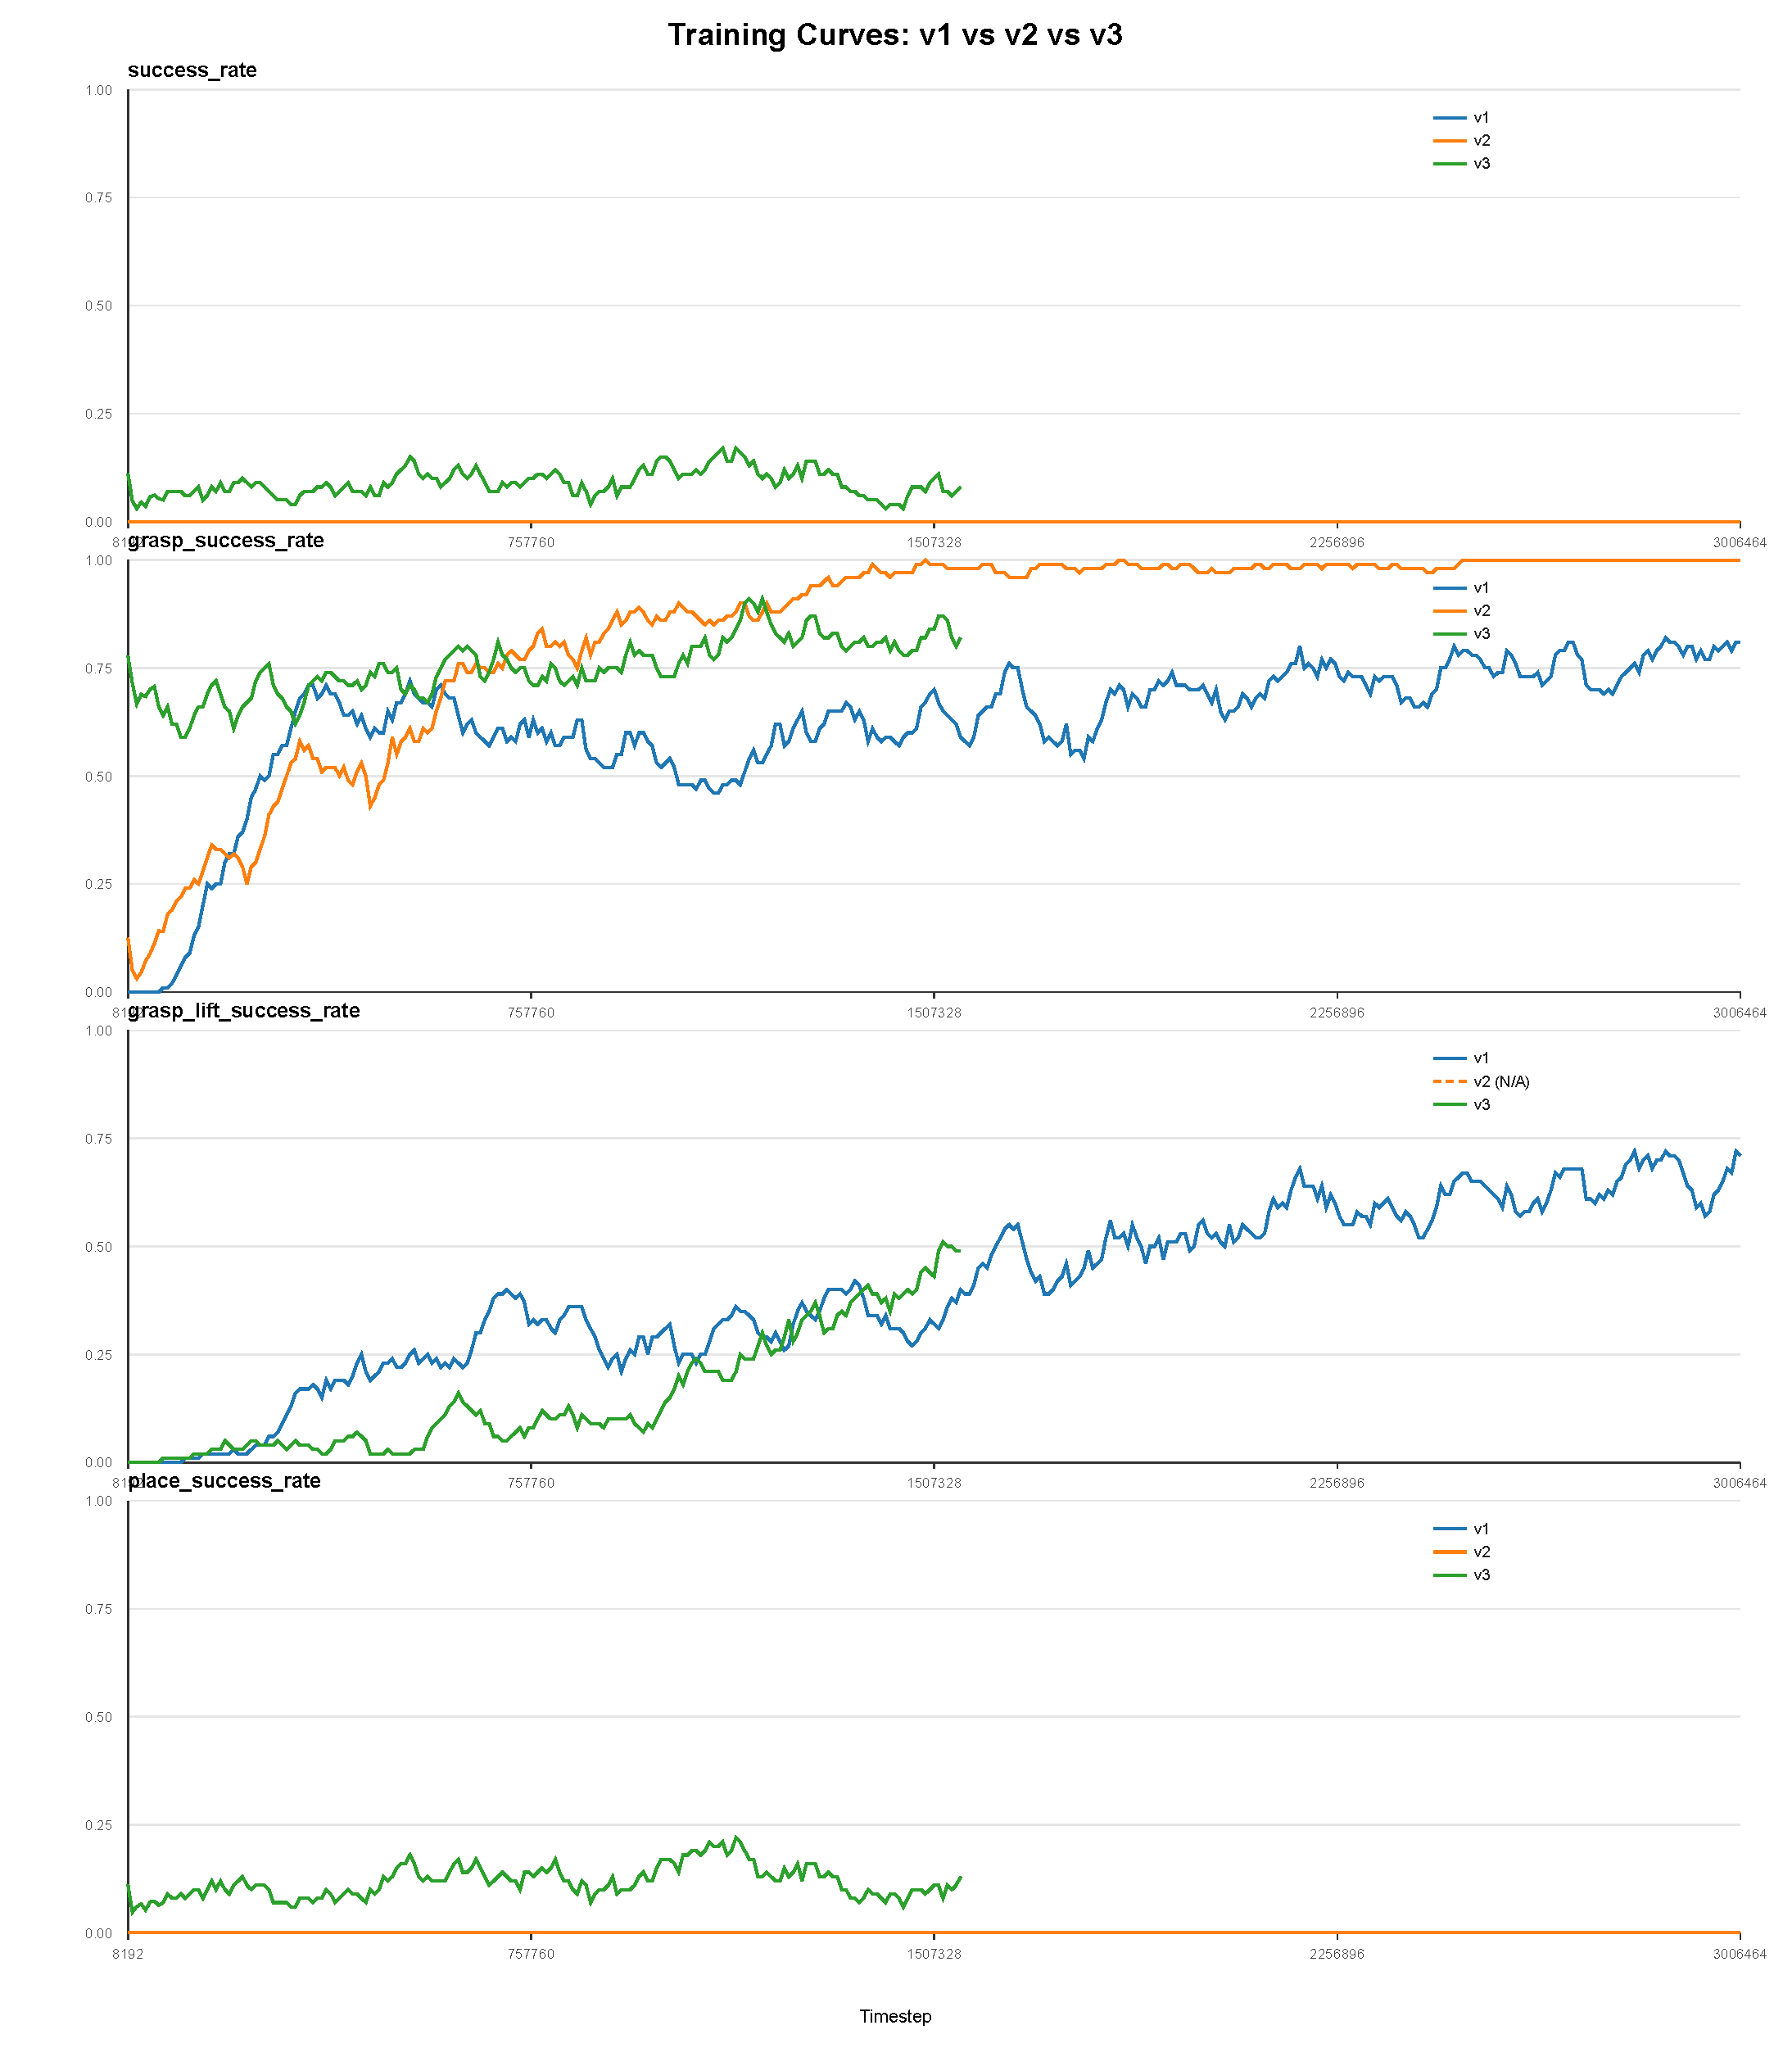
\includegraphics[width=\linewidth]{images/training_curves_v1_v2_v3.pdf}
\caption{Training curves of success-related metrics across v1, v2, and v3.}
\label{fig:success-curves}
\end{figure}

\begin{figure}[h]
\centering
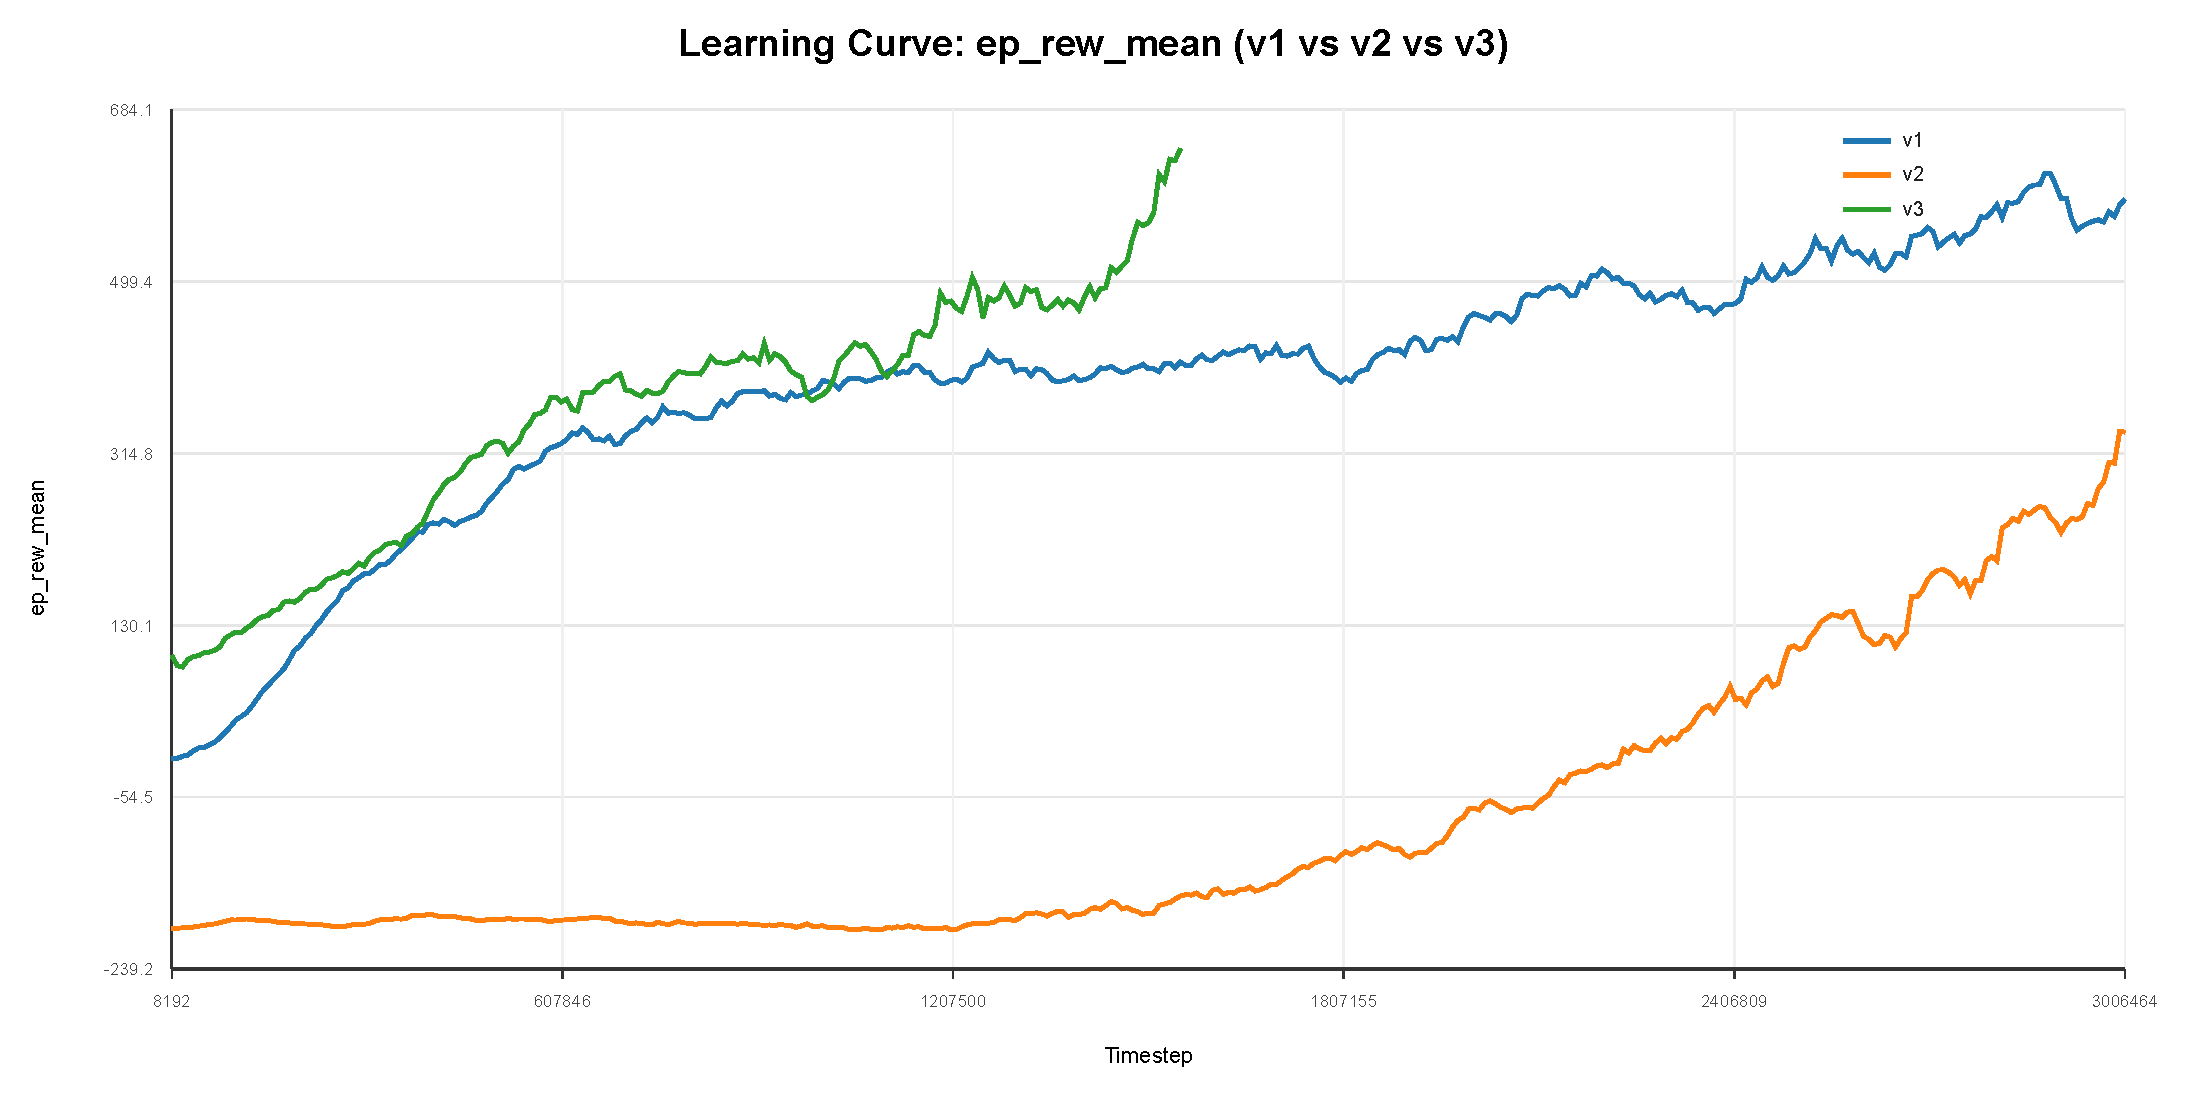
\includegraphics[width=\linewidth]{images/learning_curve_ep_rew_mean_v1_v2_v3.pdf}
\caption{Training curve of mean episode reward for v1, v2, and v3. Because the three versions use different reward formulations, these reward-scale curves are not directly comparable across versions and are shown only to illustrate within-run training trends.}
\label{fig:ep-rew-curve}
\end{figure}

\subsubsection{PPO Key Findings}
\begin{itemize}
    \item v1 and v2 both show strong grasp learning on apple-to-cab, with v2 reaching near-saturated grasp rate.
    \item v3 achieves non-zero placement and final success on apple-to-bowl, unlike v1/v2 in their reported logs.
    \item The dominant tension in v3 is not gripper timing alone but \emph{progress along the full carry}: grasp rates stay high while place and full success lag, matching a transport-and-terminal-alignment bottleneck (getting and keeping the apple in a successful bowl configuration) more than a pure ``forgot to open'' pattern. Reward engineering explicitly had to down-weight sustained hovering and up-weight bowl-directed transport, which supports reading the remaining gap as largely carry- and completion-shaped.
\end{itemize}

\subsection{SAC+HER Results}
The SAC+HER curriculum track highlights a \emph{release-dominated} failure mode that contrasts with the PPO logs:
\begin{itemize}
    \item \textbf{Bowl Phase 1B (placement-focused)} reaches \(\sim 94\%\) success, indicating that transport and bowl-level placement can be learned reliably under curriculum support.
    \item \textbf{Bowl Phase 1C (release-required)} plateaus near \(\sim 5\%\), showing that adding precise release timing sharply increases difficulty even when spatial positioning is mostly solved.
    \item \textbf{Separate cabinet-task log (not the bowl setup above):} an additional run on the cabinet environment shows promising early grasp emergence (\(\sim 11.1\%\)), then regression to low grasp rates (\(\sim 1\%-3\%\)); it illustrates transfer or curriculum fragility elsewhere but should not be read as a direct output of the bowl HER configuration in Method~B.
\end{itemize}
\noindent Thus, in these runs SAC+HER is comparatively strong at getting the apple to the bowl region under shaping and hindsight, and comparatively weak at the \emph{event} of opening and leaving the object in the success set. That is a different emphasis from PPO v3, where grasp is strong but carry-to-success remains the main metric gap.
Figures~\ref{fig:sac-her-learning-curves}, \ref{fig:sac-her-opend-reled}, and \ref{fig:sac-her-phase-annotations} provide detailed SAC+HER diagnostics oriented around release distance and curriculum transitions.

\begin{figure}[h]
\centering
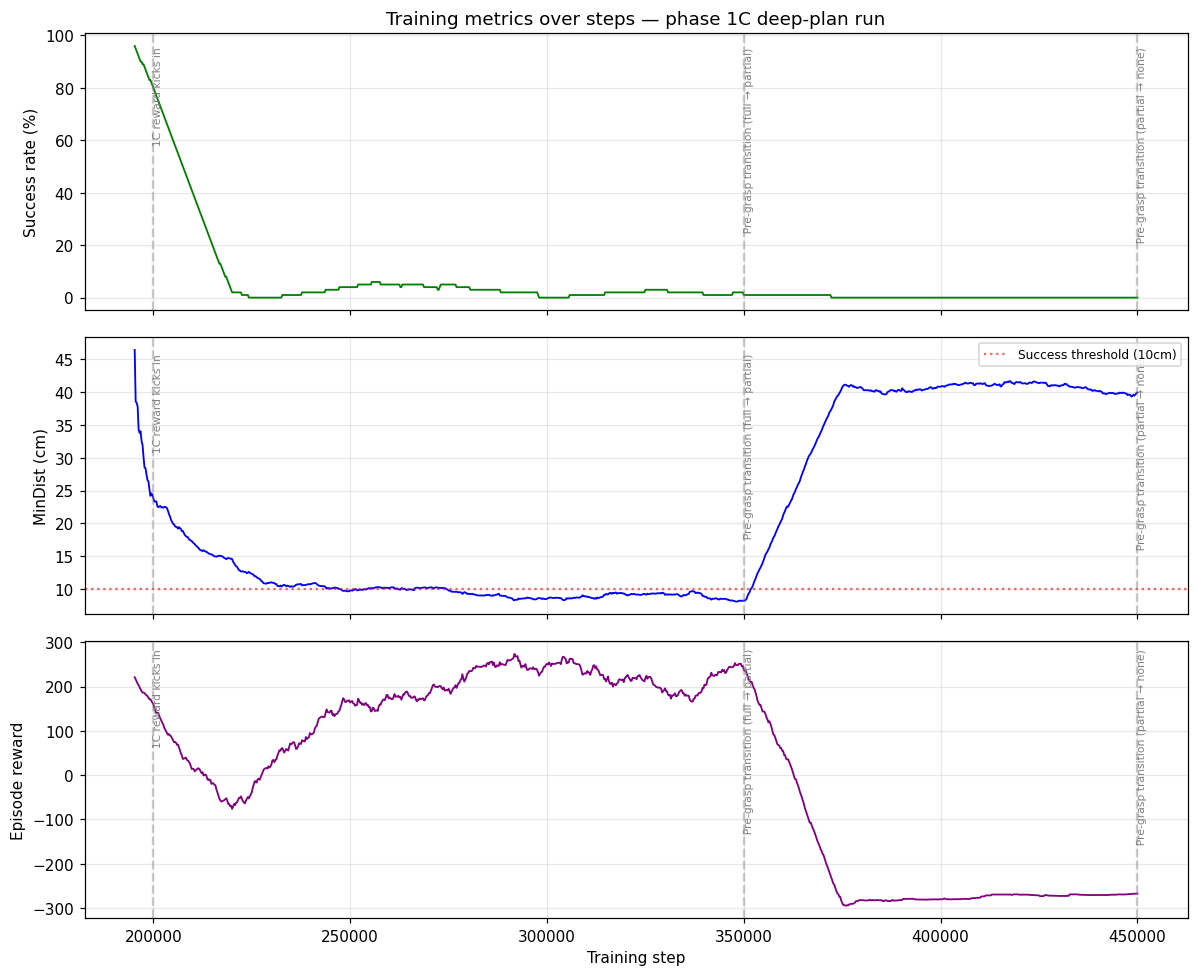
\includegraphics[width=\linewidth]{images/sac_her_learning_curves.png}
\caption{SAC+HER phase 1C deep-plan run: success rate, minimum bowl distance, and episode reward over training steps. Performance drops align with curriculum hardening (e.g.\ reward phase, pre-grasp mode, or stricter success radius), not a single knob in isolation.}
\label{fig:sac-her-learning-curves}
\end{figure}

\begin{figure}[h]
\centering
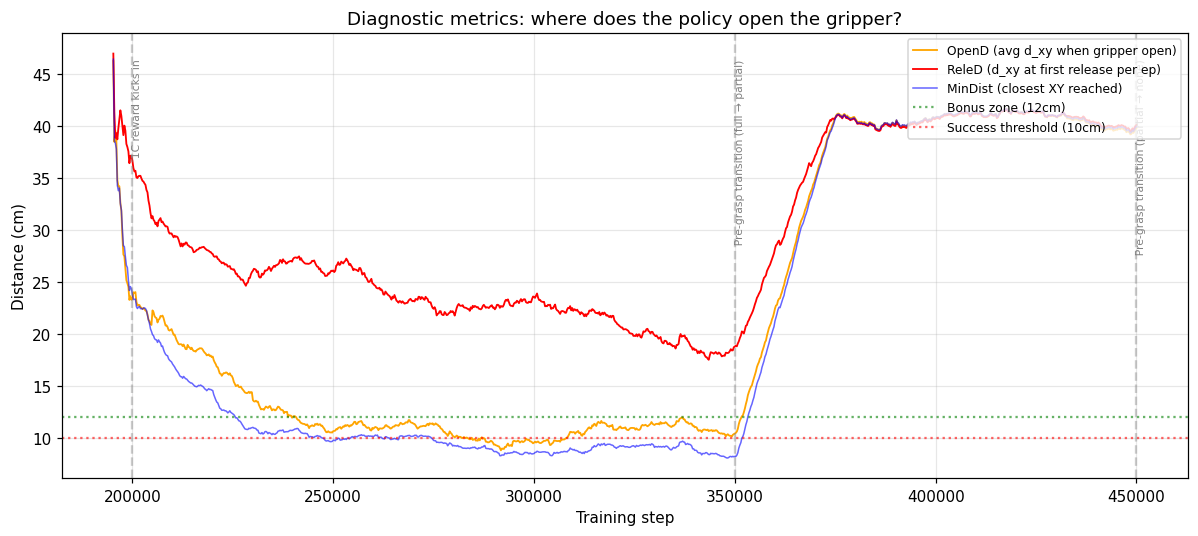
\includegraphics[width=\linewidth]{images/sac_her_opend_releD.png}
\caption{SAC+HER release diagnostics: open-distance (\texttt{OpenD}), release distance (\texttt{ReleD}), and closest approach (\texttt{MinDist}) to the bowl. The policy opens increasingly far from the success zone after transition.}
\label{fig:sac-her-opend-reled}
\end{figure}

\begin{figure}[h]
\centering
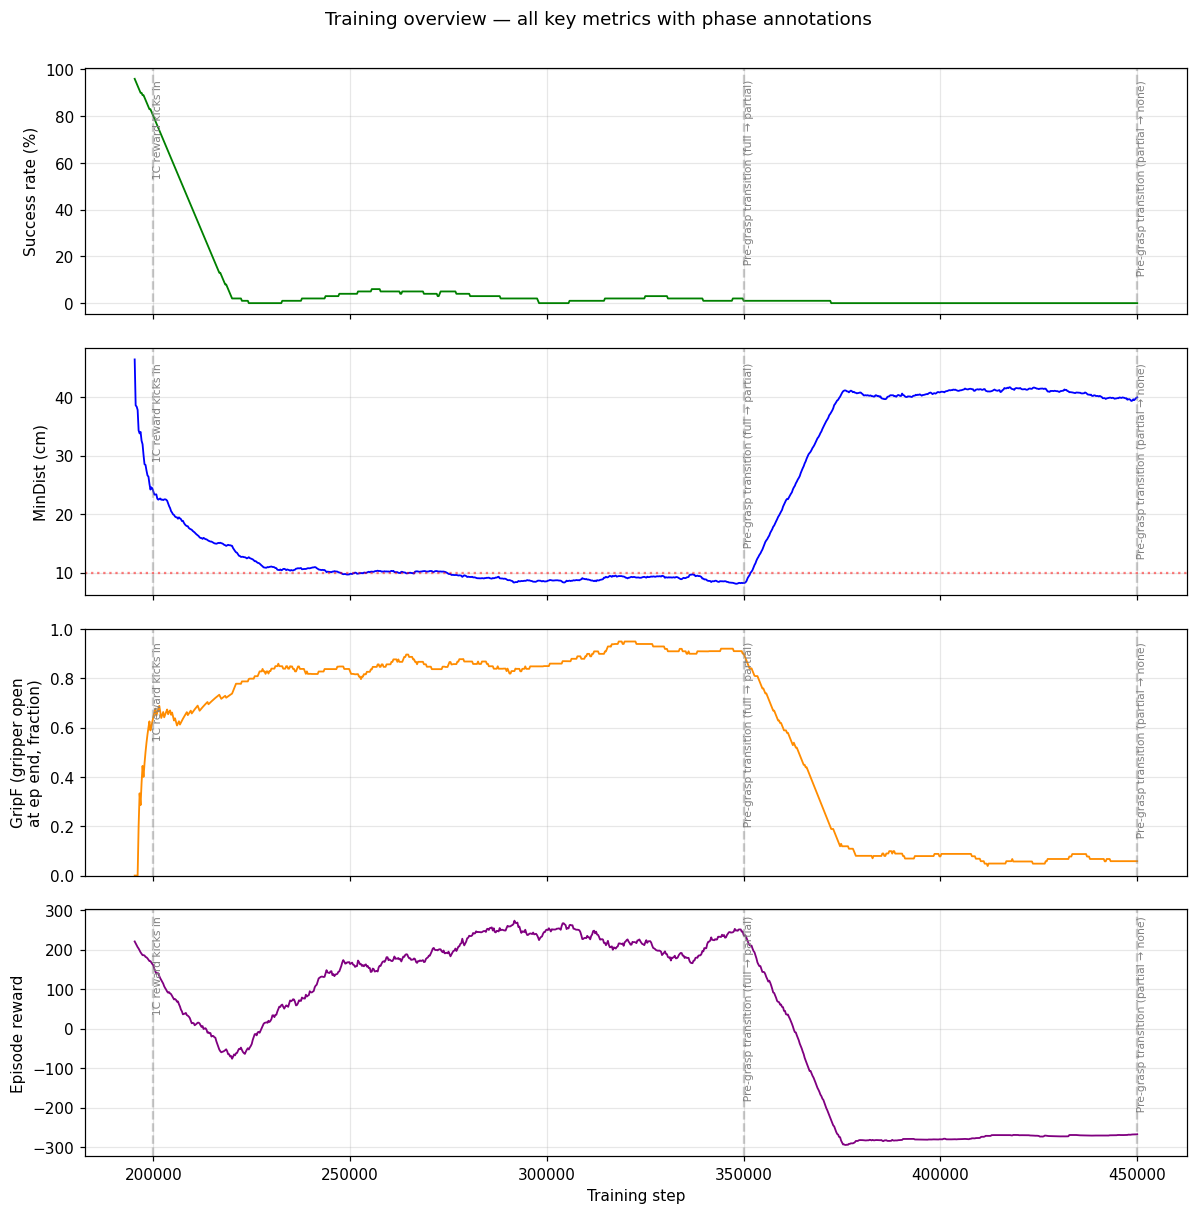
\includegraphics[width=\linewidth]{images/sac_her_phase_annotations.png}
\caption{SAC+HER integrated phase-annotated overview across key metrics. Transitions toward full difficulty (pre-grasp, reward phase, thresholds, or mobility) coincide with sharp changes in success and reward.}
\label{fig:sac-her-phase-annotations}
\end{figure}

\subsection{Cross-Method Behavioral Evidence}
Qualitative rollouts align with the split above. For PPO shaping, policies typically reach and grasp reliably; failures are often visible as incomplete or unstable \emph{carriage} into the bowl success volume (hovering, partial approach, or placement that does not meet full termination). For SAC+HER after hardening phases, the arm frequently reaches the vicinity of the bowl, yet the gripper opens in a \emph{mis-timed} or spatially offset way relative to the strict success test. So both lines show compositional gaps, but the salient video-level story is transport-leaning for PPO and release-leaning for SAC+HER in the material summarized here.

\subsection{Task Visualization}
Figure~\ref{fig:task-visualization} shows four frames from the \textbf{first six seconds} of a deterministic PPO reward-shaping \textbf{v3} evaluation rollout on apple-to-bowl (episode~0), illustrating early reach and approach. In a small set of evaluation replays, grasping succeeds yet we did not observe a full successful placement of the apple into the bowl under the task success criterion.

\begin{figure}[h]
\centering
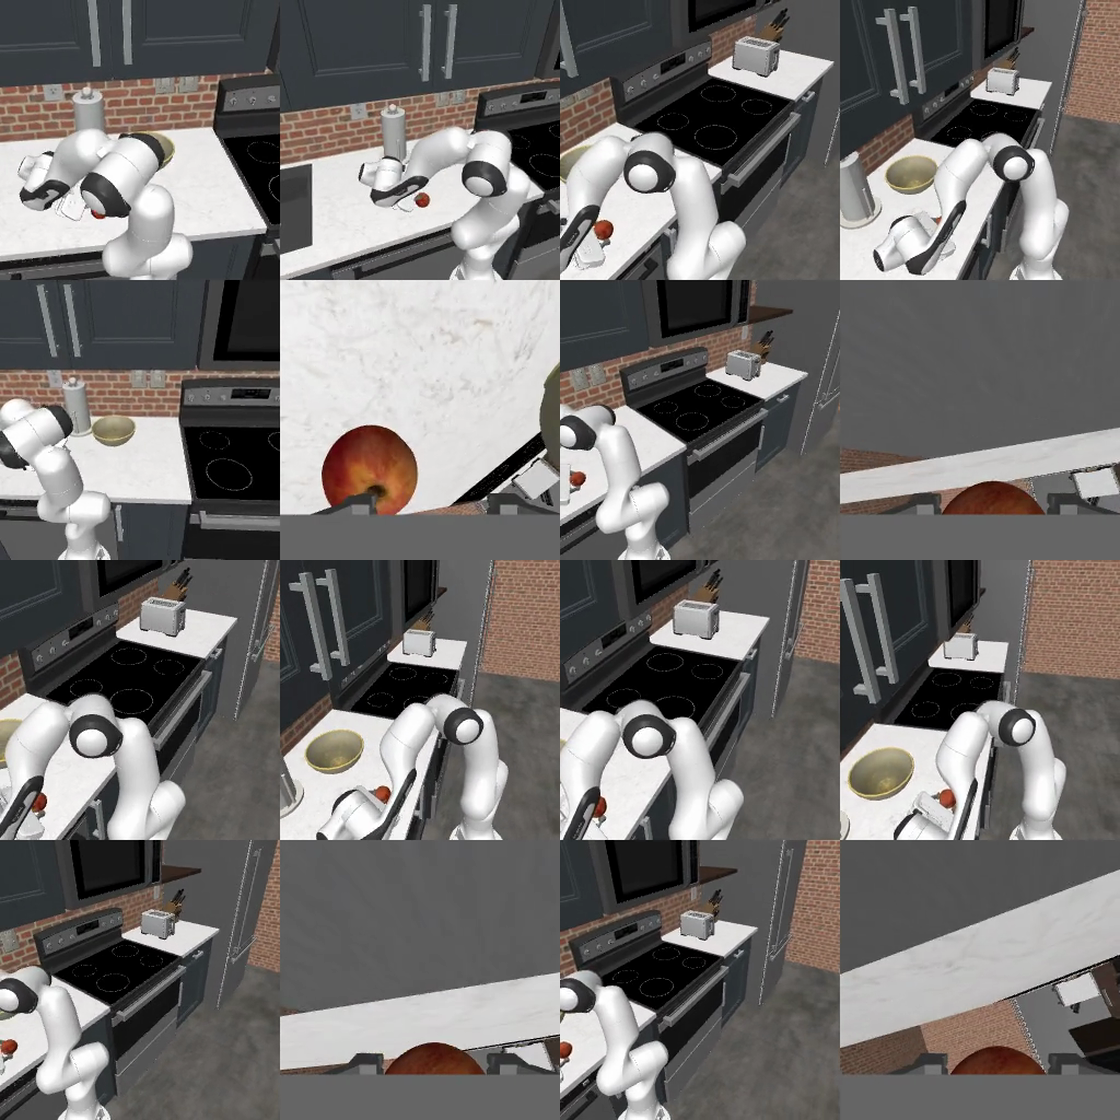
\includegraphics[width=0.85\linewidth]{images/task_visualization_v3_ep00_first6s_montage.png}
\caption{Task visualization (2$\times$2 montage): first six seconds of episode~0 for PPO shaping v3 (apple-to-bowl). Early-episode reach and approach toward the apple and workspace.}
\label{fig:task-visualization}
\end{figure}

\subsection{Unified Interpretation}
Both methods support a common \emph{task-level} lesson---pick-and-place is a chain of skills, and the chain breaks most visibly under distribution shift---but the \emph{weak link} differs:
\begin{itemize}
    \item \textbf{PPO (shaped)}: early segments (reach, grasp) saturate more easily than reliable \emph{end-to-end carry} into bowl success; reward design must fight local optima around lift and hover rather than only around release timing.
    \item \textbf{SAC+HER (curriculum)}: staged training solves much of spatial behavior, then exposes a sharp \emph{release} cliff when the objective demands an open gripper in the right place at the right time.
    \item \textbf{Shared trigger}: harder task slices (cabinet-to-bowl transfer for PPO; phase~1C and pre-grasp tightening for SAC+HER) make whichever weak link is dominant obvious in the metrics.
\end{itemize}

\section{Discussion}
\subsection{Why Both Methods Improve Early Learning}
Compared with sparse-only learning, PPO shaping and SAC+HER curriculum both provide denser supervision and produce stable progress on contact, grasp, and transport stages.

\subsection{Why Final Success Remains Limited Across Methods}
Factors apply differently to each pipeline:
\begin{enumerate}
    \item \textbf{Reward and objective shape (PPO)}: dense terms for lift, sustain, and transport must be balanced so the policy invests in bowl-directed motion rather than grasp-only or hover-heavy trajectories; mis-weighting shows up as a grasp--place--success gap even when release is not the only missing ingredient.
    \item \textbf{Event timing and credit (SAC+HER)}: opening the gripper is a short, decisive event coupled to contact physics and hindsight relabeling; when the curriculum adds explicit openness to success, credit assignment and exploration concentrate on release quality, and small policy errors appear as large success drops.
    \item \textbf{Strict termination (both)}: bowl success ties together pose, height, openness, and often clearance; any algorithm must satisfy the conjunction, but the metric gradients emphasize transport for PPO-shaped runs and release placement for SAC+HER runs in this report.
\end{enumerate}

\noindent In short, PPO logs argue for diagnosing \emph{carry and completion} first; SAC+HER logs argue for diagnosing \emph{release under curriculum} first. Neither excludes the other at the task level, but the empirical emphasis differs between the two method sections above.

\subsection{Method-Specific Strengths}
\begin{itemize}
    \item \textbf{PPO shaping}: clearer control over reward semantics and straightforward metric instrumentation.
    \item \textbf{SAC+HER curriculum}: better sample reuse and strong performance in staged subproblems.
\end{itemize}

\subsection{Limitations}
This report is based on a limited number of runs and diagnostics. It does not include a full hyperparameter sweep, controlled seed study, or significance testing; conclusions should therefore be read as empirical evidence, not definitive generalization.

\section{Conclusion}
Dense guidance improves early and middle segments of pick-and-place, yet full bowl success remains hard. The evidence here suggests \emph{different} dominant gaps for the two algorithmic choices: PPO with reward shaping chiefly struggles to close the \emph{transport and terminal-alignment} hole between strong grasp and reliable success; SAC+HER with curriculum chiefly struggles at the \emph{release} transition once spatial phases are learned. PPO v3 reaches non-zero success with grasp still ahead of place and success; SAC+HER reaches strong intermediate placement then stalls when openness is required.

The implication is not a single cross-algorithmic ``release-only'' story but a compositional task where methods allocate error to different segments. Future work should treat transport-strong and release-strong diagnostics separately: carry-aware shaping and evaluation for PPO-style training, and release-aware exploration, reward--HER consistency, and curriculum hand-offs for SAC+HER-style training.

\end{document}
